\chapter{Platforms' Inspection Mechanisms}
\label{ch:Platforms Problem}

So far we created a setup for information exchange between a group of rational agents alongside with the rationalization of the assumptions we made for our model. The next step is to define the behaviour of our authoritative entity, in our case the platform which is the social medium where agents interact and share stories with each other. Given that the platform has an overview of the whole process, we utilize this knowledge under a number of assumptions, to develop appropriate tools for our platform in order to intervene and inspect information. Our goal is to consider the properties of our network that will specify the optimal time for inspection. 

In this chapter we introduce platform's role in the sharing process model and the inspection problem. We modify the basic sequential model introduced by ~\cite{papanastasiou} in order to work for asynchronous propagation within tree structures, adding the necessary assumptions.  We continue with an analysis of the properties that emerge from those assumptions. Finally, we leverage the structure features in order to find an approximate solution for intervention and inspection of a story at proper time. 

\section{Introducing Platform in the Sharing Process}
\label{sec:platformIntro}

So far we have an ecosystem where agents share messages called \textit{stories}, as we mentioned in previous chapter, and their actions are under the assumption that are responsible individuals. This technically means that they act in order to maximize their expected utility by not sharing non trusted stories according to their judgment. Now we introduce the platform, where those individuals reside in. Examples of such entities are Facebook, Twitter, YouTube and many more, where millions of user interact and share information with each other. In our case study, platform is a \textit{super} agent providing those online services in order for agents to interact with each other. In our study, the platform observes the evolution of the propagation tree, and infers the posterior probabilities of the involved users, so as to have its own posterior belief about the validity of a story.

\begin{figure}[t]
	\centering
	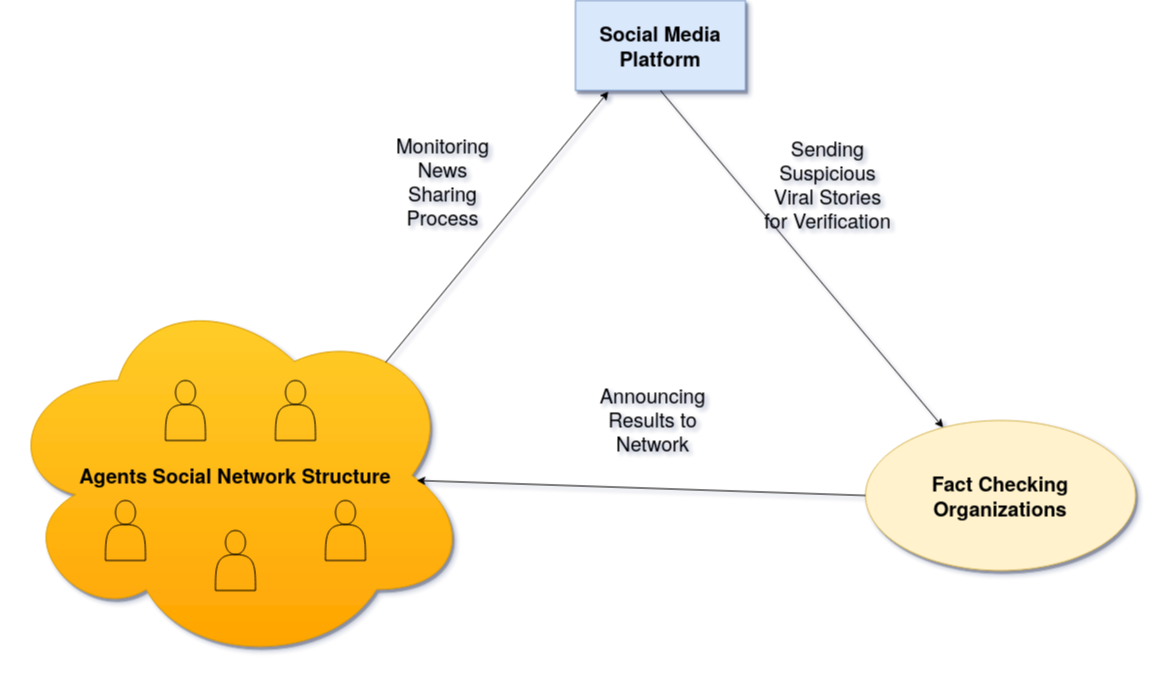
\includegraphics[width=.75\textwidth]{Figures/EntityDiagram.png}
	%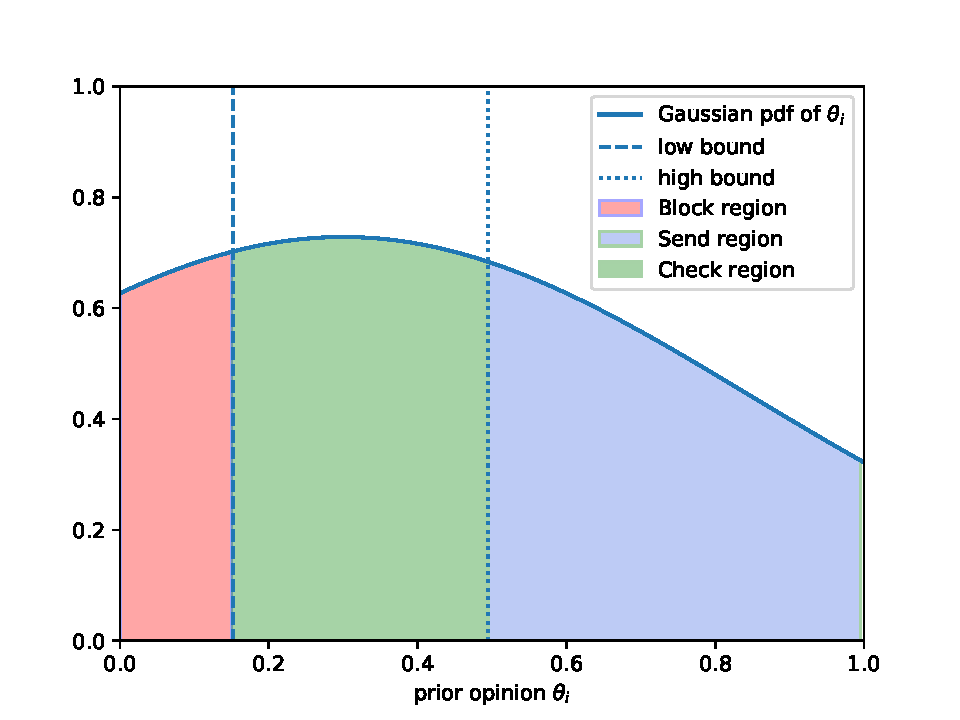
\includegraphics[width=.75\textwidth, height=.3\textheight]{Figures/Zbounds.pdf}
	
	\caption{The fact checking model of a social media service. The fact-checking process is assumed to an external service for the platform, which of course comes with a given cost for the platform. In practical scenarios, the platforms cannot conduct a fact check over stories because this would affect their policy, given that fact checking comes with a cost.}
	
	\label{fig:entityDiagram}
\end{figure}

In figure ~\ref{fig:entityDiagram} we have our ecosystem with the introduction of platform. We see that our platform monitors the activity of agents network in order to maintain a trustworthy social network of information sharing. If platform suspects that a story is shared effortless (without any inspection), then there is a global check via fact checking organizations. Afterwards, the results are announced to our network and there are two options:

\begin{itemize}
	\item If the story is validated as truthful, then this announcement leads to a sharing cascade. Additionally, the platform will receive a discounted reward for each share of the story in our network.
	\item If the story is fake, then the sharing process is terminated and the the platform will receive only a penalty for each (previous) share of the fake story, along with a fixed global-check cost. 
\end{itemize}
In our case study, we assume that the inspection yields a perfect result. This assumption holds for both agents and the authoritative entities such as the platform or fact checking partners. We also remind that this setup is easily extensible for cases where the fact checking action occurs with error. 

Another important part of our setup is the amount of privileges that such a platform possesses. We mentioned above that our platform is a super user with extra knowledge. We assume that our platform observes the creation of edges in our network without knowing if they are product of checking action or blindly sharing the story. In other words, platform observes reactions at given round $t$ from agents without knowing the exact action, i.e. if it $A_{it}=S$ or $A_{it}=C$ in round $t$. Additionally, the platform is unaware if an agent discontinued the sharing process by blocking of checking the story. More specifically, platform cannot observe the round $t$ where an agent decided to not share a story with either $A_{it}=B$ or via checking with $A_{it}=C$. This assumption reflects a real life application where a social media administrator cannot monitor if an individual user of such a service conducted a research or not in order to share information within a network. 

This brings us to a stronger assumption that makes the building block of our model.

\begin{assumption}
	The exact value of random variables $\theta_i \sim \mathcal{N} (\theta,\sigma^2)$ for each agent $i$ are hidden from platform. Platform only assumes a normal distribution $N(\theta,\sigma^2)$ for the independent sampling of prior beliefs for the agents.
\end{assumption}
The reasoning behind this assumption, that strengthens our model in order to work under uncertainty, is that we cannot predict the exact value of a prior opinion of a random agent. For example, let's assume that we have an emerging topic. In such case, most probably, we do not have prior opinions formed on the topic or even worse, we formed wrong prior opinions. Another important property this assumption has is the fact that this model is more confidential since we can work without monitoring users of such services where there are issues of private information leaks.

As we mentioned above, the platform monitors reactions of agents, more specifically, those reactions that share information from parents to children. In other words, platform increases the round from $t$ to $t+1$ whenever a node $i$ decides to share and create edges to his \textit{friends}, \textit{followers} or children (from data structure perspective). We need to decide how those agents are picked to react and choose an action at round $t$. There are two approaches for that issue:

\begin{itemize}
	\item Agents that are terminal leaves in the sharing tree are picked uniformly at random.
	\item Agents are picked with probability $(1/m)^l$ where $m$ is the amount of children that each node have (for $m$-ary trees) and $l$ is the height of node $i$ in the sharing tree.
\end{itemize}

\begin{figure}
	\definecolor {processblue}{cmyk}{0.96,0,0,0}
	\definecolor {processred}{cmyk}{0.96,0,0,0}
	\tikzstyle{c} = [thick,draw, circle, minimum size=2,top color =white ,minimum size=2, bottom color = processblue!20,processblue]
	\centering
	\begin{tikzpicture}[main/.style={c},
	level distance=15mm,
	level 1/.style={sibling distance=20mm},
	level 2/.style={sibling distance=30mm},
	level 3/.style={sibling distance=15mm},
	end/.style = {draw, circle, minimum size=2,fill,top color=white,bottom color=red!20,red},
	discovered/.style = {draw, circle, minimum size=2,fill,color = red},itria/.style={
		draw,shape border uses incircle,
		isosceles triangle,shape border rotate=90,yshift=-1.45cm}]
	\node (a)[main,label=left:{$\theta_1$}]{}[edge from parent]
	child {
		node (b) [end,label=left:{$\theta_2$}]{}
			child {
				node (t) [itria]{L}
			}
	}
	child {
		node (c)[main,label=left:{$\theta_3$}]{} 
	}
	child {
		node (d)[main,label=left:{$\theta_4$}]{} 
	};
	\draw (a) -- (b) node [->] {};
	\draw (a) -- (c) node [->] {};
	\draw (a) -- (d) node [->] {};
	\end{tikzpicture}
	\caption{An example of a ternary sharing tree where each agent is picked uniformly at random to react. The right triangle $L$ is a subtree of the sharing tree.}
	\label{fig:unbalancedCase}
\end{figure}

It is obvious that the first approach tends to create unbalanced trees in depth first manner. In figure ~\ref{fig:unbalancedCase} we see such a case. After the root decided to share the information, let's assume that node $\theta_2$ is picked with probability $1/3$, since we have a ternary propagation tree, tree, to react at round $2$. The set of leaves at that round, we call it frontier from now on, consists of nodes $\theta_3$, $\theta_4$ and the children of $\theta_2$, $D_{\theta_2}$. Because we assumed that agents are picked uniformly at random, hence the probability of picking a node on the frontier is now $1/(\mid \{\theta_3,\theta_4\} \cup D_{\theta_2}) \mid$, in case of our example it is $1/5$ since we have $3$ children of $\theta_2$ plus the nodes in level $1$. This implies that $\theta_2$ will probably will be picked, with probability $3/5$, rather than $\theta_3$ or $\theta_4$, with probability $2/5$. Moving forward in the next round, the probability of picking one node to react in the subtree $L$ will increase once again, making more likely an expansion of the sharing tree towards $L$.

On the other hand we have the second approach where the level of each node matters, hence we have that node $i$ is picked with probability $(1/m)^l$ where $m$ is the amount of children each node is assumed to have\footnote{We are using mean field analysis in our approach with an average degree for children in our tree structure. Thus we are developing this model over $m$-ary trees.} and $l$ is the level where node $i$ belongs. This approach is used to tackle down the issue that we have with unbalanced tree when we are picking uniformly at random and also it is reasonable to say that we expect from nodes who received the story earlier to react faster than freshly activated nodes in the sharing tree.

Now that have established the role of the platform, alongside with the appropriate assumptions, we proceed with the technical part and the introduction of the optimal inspection problem. 


\section{Platforms' Inspection Problem}
\label{sec:platformInspection}

Since we assumed that inspection yields a perfect outcome, it is sufficient to find one agent that inspected the element. If an agent that inspects the story and decides to share that means he found the story truthful. Because we assumed that the result is irrefutable, the announcement of that the story is truthful will trigger an information cascade in the sharing tree, and each sharing action afterwards will increase the discounted reward that platform receives, i.e. advertise revenue or another monetization strategy that is benefit from sharing content. Apart from the agents' private inspections (fact-checks) for the type of a story, the platform may also intervene by requesting a global fact-check (e.g., from an external third-party fact-checking service) and then communicating the result of this inspection to the entire community.  

On the other hand, we have agents that are not reacting, and we cannot presume if the chose $A_{it} = C$ or $B$ as an action, as we specified in section ~\ref{sec:platformIntro}. An agent might block a story either with or without inspection and that is hidden from platform since it does not posses the exact value of $\theta$ for each agent nor it is clear if the agent inspected or plainly blocked the story. Thus it is important for the platform to estimate the probability that some agent received the story and decided to inspect and block it. Once again, this event is sufficient enough since inspection is perfect. The platform can also utilize the probability of that event and dispute the validity of that story via fact checking organizations. We assume that the intervention of the platform in the evolution of the emergent story via fact-checking comes with a cost $K_p$. Now that we established those two warning mechanisms for global check, we provide two propositions in order to calculate the probabilities of those events.

\begin{prop}
	Let $T$ be a sharing tree and $m=y$ is the story that propagates in $T$. Then the platform's belief there exist an agent $i$ and $A_{it}=C$ at some round $t$ in $T$, under the assumption that platform observes independent random experiments over agents, is: 
	$$r_T = 1-\mathbb{P}_{pT} \{\forall i \in \mathcal{V}_{T}: A_{it}=S \mid H_i,m=y \} =  1 - \displaystyle \prod\limits_{\substack{k = 0 \\ i \in \mathcal{V}_{T}}}^{t-1} \mathbb{P} [A_{ik} = S_{ik}^p] $$ where $\mathcal{V}_{T}$ are the set of nodes of $T$, respectively.
	\label{prop:GreenProb}
\end{prop}

Before we begin with the proof of proposition ~\ref{prop:GreenProb}, it is important to mention that time is irrelevant in that equation since we can rearrange the sequence of shares and agents id's in order. We keep the annotation of $A_{it}$ though to avoid \textit{polluting} this thesis with unnecessary notations. That being said, we only use the next definition in order to specify the platform's belief over agents' $i$ action:

\begin{definition}
	For each action $A_{it} = \{B,C,S \}$ of an agent $i$ in round $t$, we define the probabilities $B_{it}^p$, $C_{it}^p$ , $S_{it}^p$ that estimate the platform's perception over the probabilities $B_{it}$, $C_{it}$ , $S_{it}$ for each action respectively.
\end{definition}

\begin{proof}{(Proposition ~\ref{prop:GreenProb})}
	We need to calculate the probability of the event that at least one agent chose C given that we have a sharing $T$ and a story claiming $m=y$. Let this probability be $r_T$. We have that $ r_T=\mathbb{P}_{pT} \{\exists i \in \mathcal{V}_{T}: A_{it}=C \mid T,m=y \} = 1-\mathbb{P}_{pT} \{\forall i \in \mathcal{V}_{T}: A_{it}=S \mid T,m=y \}$. The last equality is equivalent, since the worst case scenario is that none inspected the story and chose to share, in other words $A_{it}=S$, $\forall i \in  \mathcal{V}_{T}$. Since we assumed that events are independent the probability $r_T$ is the product of all those independent experiments, thus $ r_T = 1-\mathbb{P}_{pT} \{\forall i \in \mathcal{V}_{T}: A_{it}=S \mid T,m=y \} \approx 1 - S_{00}^p S_{11}^p S_{22}^p . . .S_{i(t-1)}^p$ where we rearranged agents id's to match the round at where they reacted throughout the propagation process due to the fact that actions are calculated independently. Thus we have that $r_T =  1 - \displaystyle \prod\limits_{\substack{k = 0 \\ i \in \mathcal{V}_{T}}}^{t-1} \mathbb{P} [A_{ik} = S_{ik}^p]$, where $S_{ik}^p$ is platform's perceived value that agent $i$ chose $S$ in round $t$. 
\end{proof}
This value is the platform's posterior belief, just before the $t$-th round of sharing, that at least one of the internal nodes actually conducted a check. Additionally, the above calculation provides us with a warning indicator that approximates the approach followed in ~\cite{papanastasiou}, where platform has a normalized belief $q_p$ that a story is fake, based on the evolution of a sharing process in a path. This approach cannot be used in the case where we have a tree structure since there are nodes that we are unsure of their reaction. To further understand this issue, let's assume that we have an $m$-ary tree and there is a node in first level that did not react after $m+t_0$ rounds. If the value of $t_0$ is large enough at a point where the process evolved in lower depths, then it is safe to assume that agent $i$ either rejected the story by choosing $B$ or inspected the story and disclosed it's validity with $C$. It is obvious that there is a challenge in order to calculate this probability since we need to take into account the fact that the agent's reaction concerning shares are partially hidden. The next proposition calculates the existence of such an agent, more specifically, the probability that at least one agent inspected the story and found it fake.

\begin{prop}
	Let $T$ be an $k$-ary sharing tree and $m=y$ is the story that propagates in $T$. Then the platform's belief that a terminal node $i$ blocked the story $m$ by inspecting it, $A_{it}=C$, in round $t$ is:
	$$ n_{it} =  [1-(1/k)^{l_i}]^{t-t_i} (1/k)^{l_i} \frac{C_{it}^p}{B_{it}^p+C_{it}^p}$$
	where $l_i$ is the level of node $i$ in $T$ and $t_i$ is the round where $i$ received the story.
\end{prop}

\begin{proof}
	Let $i$ be a random node of $T$ and $l_i > 0$ \footnote{We do not bother proving the proposition for root since it holds trivially.} its' depth in it. We will prove the claim by induction over $t-t_i$. For $t-t_i = 0$, which means after the first time that node $i$ was candidate to react, there are to cases:
	\begin{itemize}
		\item With probability $1-(1/k)^{l_i}$, node $i$ it is not picked to react at current round.
		\item With probability $(1/k)^{l_i}$, node $i$ reacts in that round.
	\end{itemize} 
In case where the node is picked to react, the probability that this node will inspect the story and then decide to block it because it is fake, is equal to $\frac{C_{it}^p}{B_{it}^p+C_{it}^p}$. Thus we have that: $$n_{i,t_i} = (1/k)^{l_i} \frac{C_{it}^p}{B_{it}^p+C_{it}^p}$$
after the first round that $i$ was candidate to react and it was picked for that round. On the other hand, if we move at the next round where $i$ is once again candidate to react, then the probability that he will react in $t-t_i = 1$ is: $$n_{i,t_i+1} = P\{\text{did not react in previous round\} P\{ \text{reacts in t round with C}\}} = $$
$$[1-(1/k)^{l_i}] (1/k)^{l_i} \frac{C_{it}^p}{B_{it}^p+C_{it}^p}$$ Assuming the claim holds for $t-t_i$, we can easily prove that it holds for $t-t_i+1$ as well.
\end{proof}

\section{Optimization Criterion for Inspection Time}
\label{sec:optimize}

In this section we develop an optimization criterion based on utility maximizing approach as in \cite{papanastasiou}. Recall that we developed a model where the agents are socially responsible, which means that they share only truthful stories and also aim to maximize their utility. We assume that it is to the interest of the platform to forbid the propagation of fake stories, i.e. such platforms try to maintain their reliability in order to form a profitable model from advertisement revenue. In each round $t$, the platform observes an activation of a node in the sharing tree. This means that rounds represent a counter for the amount of nodes that reacted throughout the sharing process. At each round, and according it's belief for the validity of the story, platform can perform a global check if it suspects that the story is fake and can cause damage to it's credibility. In case where platform believes that the story is truthful we do not have any interruption of the story. 

In order to develop a criterion to calculated the existence of an optimal time to interrupt the process in order to avoid further damage that un checked shares will cause, we develop a utility maximizing scheme. We assume that if the story is fake, then for each successful share platform receives penalty $P$. For each successful share of a truthful story, the platform will receive a discounted reward $R$, with a discount factor $\delta < 1$ that is affected by the depth of the sharing process. The discount factor rationalization is that freshly shares are more relevant in order to form an opinion over the validity of our story. If platform decides to intervene in order to check the validity of a story, this action occurs with a cost $K_p$, and the this decision is once and for all. This means that after the announcement of the results, we have two cases. If the current story is fake, then the process ends with the appropriate penalties for each share, while if it is truthful, an information cascade triggers and platform will collect all future discounted rewards. 

Platform determines its' policy by estimating the utility of the sharing tree and the option of inspecting or not is viable respectively. At each round $t$, the process already created a sharing tree $T$. Therefore, we have an \textit{observed} utility that either we will receive penalty if the story is fake or collect reward otherwise. We define the utility that platform gains, for each agent $i$ in round $t$, as:

\begin{equation}
g_{pT} (V) = 
\begin{cases}
P, & \text{w.p. } S_{it}q_{pT} \textit{ if } V=F \\
R, & \text{w.p. } (S_{it}+C_{it})q_{pT} \textit{ if } V=T\\
0, & \text{else} \\
\end{cases}
\label{eq:platUtility}
\end{equation}

Assuming that platforms belief, that the story is fake, is $q_{pT}$, we have the following lemma for the observed utility of our platform:

\begin{lemma}
	The expected observed discounted utility that platform gains from a sharing tree $T$ is:
	$$ O_{p}(T) = \sum_{i \in \mathcal{V}_{T}}  \delta^{l_i} \left[ P ( S_{it}^p q_{pT} ) + R ( S_{it}^p+C_{it}^p)q_{pT}  \right]$$ where $l_i$ is the depth that agent $i$ belongs and $\mathcal{V}_{T}$ is the set of nodes/agents that belong in $T$.
\end{lemma} 

\begin{proof}
	Similarly to proposition ~\ref{prop:ExpUtility}, we have that:
	$$ O_{p}(T) =  \mathbb{E} [g_{pT} (V)]_{\forall i \in \mathcal{V}_{T}, V \in \{T,F \}}  $$
	Thus, for each internal node that we already observed its reaction, we receive a discounted reward in case it successfully shared the story. In case an internal node shares a fake story, and assuming platform's belief that the story is fake equals to $q_{pT}$, it comes with penalty $P$. According to equation ~\ref{eq:platUtility}:
	$$ O_{p}(T) =  \mathbb{E} [g_{pT} (V)]_{\forall i \in \mathcal{V}_{T}, V \in \{T,F \}} = \sum_{i \in \mathcal{V}_{T}}  \delta^{l_i} \left[ p ( S_{it}^p q_{pT} ) + r ( S_{it}^p+C_{it}^p)q_{pT}  \right]$$
	 
\end{proof}

Let's assume that we observe a sharing tree $T$ and define the frontier $\mathcal{F}$, that is a subgraph of $T$, as those nodes that are leaves of $T$ (candidates to react). Then we can calculate the expected utility that we will gain with the addition/s of nodes that belong in frontier. Let's assume that node $j$ will react and enter in the sharing tree such $T \cup \{j\}$. In worst case scenario, where the story is fake, we expect from the same tree, a penalty for each descendant of $j$. We have two possible policies, to make a global check, annotated as $\mathcal{C}$, and collect reward/penalty or to let the process continue, annotated as $\mathcal{E}$, and reevaluate the expected utility once again. If the platforms' belief that the story is fake equals to $q_{pT}$ then the expected discounted utility gained from subtree $T'$ if platform chooses to global check, is: 
$$ (\delta^{l_i} R + \delta^{l_i+1} k R + \delta^{l_i+2} k^2 R+...) (1-q_{pT}) - K_p $$
where $K_p$ is the negative utility gained because the cost of inspection. If $\delta k <1 $ we conclude that:
$$ U_{\mathcal{C}} =\delta^{l_i} (R+ \delta k R+\delta^2 k^2 R+...)(1-q_{pT}) - K_p = \delta^{l_i}(1-q_{pT}) \frac{R}{1-\delta k}-K_p$$
Observe that this is the anticipated utility gained only by one agent $j \in \mathcal{F}$. If we want to in account every other agent $j$ in frontier we sum up the anticipated costs and we have:

$$ U_{\mathcal{C}} = \sum_{j \in \mathcal{F}} \delta^{l_j+t}(1-q_{pT}) \frac{R}{1-\delta k}-K_p$$

Now let us discuss the utility that the platform will receive if it decides that it will not intercept the sharing process. According to that strategy, $\mathcal{E}$, we have the next probable outcomes:

\begin{itemize}
	\item With probability $C_{it}$, agent $i$ checks and decide to only share a truthful story and platform collects reward.
	\item With probability $(1-q_{pT}) S_{it}$, agent $i$ shares a truthful story and platform collects reward.
	\item With probability $q_{pT} S_{it}$, agent $i$ shares a fake story and platform receives penalty.
\end{itemize}

Then, the utility we gain from agent $i$, if the platform decides to $\mathcal{E}$, is given by the equation bellow:
$$C_{it}(1-q_{pt})R + S_{it}(1-q_{pT})R + S_{it} q_{pT} P$$
Observe that the reaction of agent $i$ creates a subtree $T'$ with node $i$ as root. Then we have the recursive formula for the discounted anticipated utility that will grow exponentially and make the calculations complex. It is obvious that it is not feasible to calculate the utility that way for two main reasons. First reason is the complexity of calculations and the fact that is hard to find a closed form type for that expected utility in order to maximize it. Secondly, the platform's belief is changing while the depth increases and this formula should recalculate $q_{pT} $ at each step which increases the complexity even more.

In order to deal with that problem, we propose the next approximation method. Suppose that platform decided already the validity of the story at round $t$. Then we have two probable cases where:

\begin{itemize}
	\item The story is fake with probability $q_{pT}$ and platform chooses strategy $\mathcal{E}$.
	\item The story is true, following the same strategy.
\end{itemize}
This modification simplifies the calculations by breaking down the problem in two different cases. Let us see what happens in the case where platform decides that the story is fake. There is  only one way that fake stories will propagate after the platform decides to let the propagation evolve and it is only if an agent decides to share without check, namely $S_{ih}$. Notice that if he decided to check the story given that platform believes it is fake, implies that the agent will discontinue the propagation. So we have that the utility in that case is:
$$ \sum_{t=0}^\infty \delta^{l_j+t} \left[ S_{l_j+t} k^t P \right] $$
where $l_j$ is the depth that agent $j$ belongs, $\mathcal{T}_j$ is the subtree, rooted on agent $j$ that belongs in frontier and $\delta$ is the discount factor. If the platform decides that a story is true over a propagation tree $T$, then the story propagates with two ways. A story can be sent to the next level in the tree with $S$ or $C$ action since it is true and agents even when fact-checking it, will share it. Therefore, the probability that a story is shared equals to $(1-B_{it})$. This observation simplifies things since it is easier to express the monotonicity of the expression bellow. For that policy, we have that the next equation that expresses that utility:

$$ U_t^A = \sum_{t=0}^\infty \delta^{l_j+t} \left[ (1-B_{l_j+t}) k^t R  \right]$$where $\mathcal{T}_j$ is the subtree, rooted on agent $j$ that belongs in frontier.
Now we are ready to collect those expressions in the next proposition that gives a formula for the platforms utility if it lets the propagation evolve.


\begin{prop}
	The anticipated utility that platform gains if it decided to let the news sharing process evolve, for an agent $ j \in \mathcal{F}$ in frontier is:
	
	$$ U_f^A = \sum_{t=0}^\infty \delta^{l_j+t} \left[ S_{l_j+t} k^t P \right] $$for fake stories and
	 $$ U_t^A =\sum_{t=0}^\infty \delta^{l_j+t} \left[ (1-B_{l_j+t}) k^t R  \right]$$for truthful.
\end{prop} 
Both of the above values will express the utility the platform gains for each agent for a sub-tree created in the frontier, rooted at agent $j$. This means we get the appropriate utility from agent $j$, discounted by $\delta^{l_j}$, plus the corresponding discounted utility of his $k$ descendants and so on. Before we find the boundaries, we collect the above quantities in order to form the final expression of the platforms expected discounted utility:
$$ U_p = O_p (T) + A_p (T)$$
where the anticipated utility of our propagation tree network $T$ is:


\begin{equation}
U_p(T) = 
\begin{cases}
 &  O_p (T)+U_{\mathcal{C}}(T) \text{ , Global-check } \mathcal{C}\\
 &  O_p (T)+U_{\mathcal{E}}(T) \text{ , Let-evolve } \mathcal{E}\\
\end{cases}
\label{eq:utilsPlat}
\end{equation}


Now remains the issue of limits. As it was previously mentioned, for each agent in the frontier, in order to calculate the anticipated utility we have to calculate the probabilities of $S$ and $B$ indefinitely. In order to deal with that, we need convergence for $U_f^A$ and $U_t^A$. The next proposition uses the monotinicity of probabilities $S$ and $B$ in order to bound those values.

\begin{prop}
	For the anticipated utilities over fake and truthful news respectively, it holds that:
	$$ U_f^A  < \delta^{l_j} S_{l_j} \frac{P}{1-\delta k} = \overline{U}_f^A$$for fake stories and
	$$ \delta^{l_j}(1-B_{l_j}) \frac{R}{1-\delta k} = \underline{U}_t^A < U_t^A  $$for truthful, where $j$ is the corresponding root agent that belongs in frontier.
	\label{prop:firstThresholds}
\end{prop}

\begin{proof}
	We have from corollary ~\ref{cor:SBBOUNDS} that $S_{l_j}$ probability is increasing in depth ${l_j}$, thus we have that $(S_{l_j} < S_{l_i}$ in every level $l_i$ lower than $l_j$. Thus we have that:
	
	$$ U_f^A = \delta^{l_j} (P S_{(l_j)} + \delta k PS_{(l_j + 1)} +\delta^2 k^2 P S_{(l_j + 2)}+...) < $$ $$ \delta^{l_j} (P S_{(l_j)} + \delta k PS_{(l_j)}+\delta^2 k^2 P S_{j(l_j)}+...) = \delta^{l_j}S_{l_j} \frac{P}{1-\delta k}$$when $P<0$
	
	Respectively, we have that $B$ is decreasing in depth. Thus $(1-B_{l_i}) > (1-B_{l_j})$ for every level $l_j$ lower than $l_i$. In similar manner we can restrict, the anticipated utility for the case a true story, such that:
	
	$$U_t^A = \delta^{l_j} (R (1-B_{(l_j)}) + \delta k R (1-B_{j(l_j + 1)}) +\delta^2 k^2 R (1-B_{(l_j + 2)})+...) > $$ $$ \delta^{l_j} (R (1-B_{(l_j)}) + \delta k R(1-B_{(l_j)}) +\delta^2 k^2 R (1-B_{j(l_j)}) +...) = \delta^{l_j}(1-B_{l_j}) \frac{R}{1-\delta k} $$ 	
\end{proof}
In the last proposition, we use the probabilities of root $j$ in the frontier, in order to bound the geometric series. This is an important step, which will help in advance to find a closed type equation for the anticipated utility. This allows the platform to make a better prediction instead of letting the process continue up to the point that agents propagation process arrive at some depth $T_c$ where they all choose to share.

\iffalse
The next proposition calculates upper and lower thresholds for the values $U_f^A$ and $U_t^A$ respectively. Those values and their existence depends on the starting state of the process and the perceived values of proposition ~\ref{prop:ZBounds}. Additionally, those bounds reduce the complexity of the calculations, since we do not go further in each subtree, in order to calculate the probabilities $B_{it},C_{it},S_{it}$.

\begin{prop}
	Depending on the initial state of thresholds of proposition ~\ref{prop:ZBounds}, it holds that:
	$$\underline{U}_f^A < U_f^A  < \overline{U}_f^A =  \delta^{l_j}B_{l_j} \frac{P}{1-\delta k}$$for fake stories and
	$$ \delta^{l_j}(1-S_{l_j}) \frac{R}{1-\delta k} =\underline{U}_t^A < U_t^A <  \overline{U}_t^A$$for truthful.
The above thresholds hold only when $S_{i0} > B_{i0}$ at the initial state.
	
\end{prop}


\begin{proof}
	\[
\delta^{l_j} B_{l_j} / (1 - k\delta) 
< \delta^{l_j} S_{l_j} / (1 - k\delta)
\Leftrightarrow
\delta^{l_j} P B_{l_j} / (1 - k\delta) 
> \delta^{l_j} P S_{l_j} / (1 - k\delta)
\]
	
The proof of this claim is similar with the proposition ~\ref{prop:firstThresholds}. We we only bound the values $(1-S_{l_i})$ and $(1-B_{l_i})$ with the constraint we have in the proposition that $S_{i0} > B_{i0}$ and the limits of geometric series are derived with the same manner. First, we have that initial $S_{i0} > B_{i0}$, thus we have that $1-S_{i0} < 1-B_{i0}$. From the monotonicity of those probabilities we have that:
\begin{align}
\begin{split}
1-S_{i1} < 1-B_{i1} \\
1-S_{i2} < 1-B_{i2} \\
... \\
1-S_{ih} < 1-B_{ih}
\end{split}
\end{align}
This proves the claim since we can bound all the terms from each inequality, such that:	
$$U_f^A = \delta^{l_j} (P S_{(l_j)} + \delta k PS_{(l_j + 1)} +\delta^2 k^2 P S_{(l_j + 2)}+...) >  $$ $$\delta^{l_j} (P B_{(l_j)} + \delta k PB_{(l_j + 1)} +\delta^2 k^2 P B_{(l_j + 2)}+...) >$$
$$\delta^{l_j} (P B_{(0)} + \delta k PB_{(0)} +\delta^2 k^2 P B_{(0)}+...) = \delta^{l_j}B_{0} \frac{P}{1-\delta k} $$
and
$$U_t^A = \delta^{l_j} (R (1-B_{(l_j)}) + \delta k R (1-B_{j(l_j + 1)}) +\delta^2 k^2 R (1-B_{(l_j + 2)})+...) >  $$ $$\delta^{l_j} (R (1-S_{(l_j)}) + \delta k R (1-S_{(l_j + 1)}) +\delta^2 k^2 R (1-S_{(l_j + 2)})+...)	>$$
$$\delta^{l_j} (R (1-S_{(l_j)}) + \delta k R (1-S_{(l_j)}) +\delta^2 k^2 R (1-S_{(l_j)})+...) = \delta^{l_j}(1-S_{l_j}) \frac{R}{1-\delta k}	$$
\end{proof}



Notice that the above boundaries are not that tight in terms of how they enclose the actual values. They also depend on the initial state of the system which is not necessary useful from algorithmic perspective. Their significance is on the time complexity and the fact that include all the characteristics of the propagation process, the discount factor, the platforms belief, the depth of the tree and the breadth (the average neighborhood size which is $k$).
\fi
\begin{figure}
	\definecolor {processblue}{cmyk}{0.96,0,0,0}
	\definecolor {processred}{cmyk}{0.96,0,0,0}
	\tikzstyle{c} = [thick,draw, circle, minimum size=2,top color =white ,minimum size=2, bottom color = processblue!20,processblue]
	\centering
	\begin{tikzpicture}[main/.style={c},
	level distance=15mm,
	level 1/.style={sibling distance=20mm},
	level 2/.style={sibling distance=30mm},
	level 3/.style={sibling distance=15mm},
	end/.style = {draw, circle, minimum size=2,fill,top color=white,bottom color=red!20,red},
	discovered/.style = {draw, circle, minimum size=2,fill,color = red},itria/.style={
		draw,shape border uses incircle,
		isosceles triangle,shape border rotate=90,yshift=-1.45cm}]
	\node (a)[main,label=left:{$\theta_1$}]{}[edge from parent]
	child {
		node (b) [main,label=left:{$\theta_2$}]{}
		child {
			node (t) [itria]{$T_1$}
		}
	}
	child {
		node (c)[main,label=left:{$\theta_3$}]{} 
		child {
			node (t) [itria]{$T_2$}
		}
	};
	\draw (a) -- (b) node [->] {};
	\draw (a) -- (c) node [->] {};
	\end{tikzpicture}
	\caption{Evolution of platforms' utility on a binary propagation tree. On round $1$, the utility of agent was already evaluated and the policy was chosen by platform. This is a greedy approach of finding the optimal policy.}
	\label{fig:optSubProp}
\end{figure}

In order to choose policy, we can restrict the calculation on future rewards/penalties and the total inspection cost. Based on the two policies we can compare the anticipated utility for both of them and find the first round where the sign changes. Therefore, it is sufficient to observe the anticipated utility, for both policies, in order to decide whether to terminate the process. If begin at round $t=0$, where the first agent, $1$ with $\theta_1$, has already reacted and we have to calculate the anticipated utility that platform will gain from his children. We assume that the average neighbor size is $k=2$. Then we have that:
$$U_p (T) = O_p (T) + A_p (T) = O_{p}(\{\theta_1\})  + A_p(\{\theta_1\})$$where in that case the $T$ consists only the first node $\theta_1$ and $A_p(\{\theta_1\}) = U_{\mathcal{E}} - U_{\mathcal{C}}$.
	
Whenever a node reacts, it adds $k$ new nodes in frontier and removes the node that reacted in the previous round as we see in figure ~\ref{fig:optSubProp}. In our case, since $k=2$, we get $2$ new nodes in the first level. Since the observed cost is: 
$$\sum_{i \in \mathcal{V}_{T}}  \delta^{l_i} \left[ P ( S_{it}^p q_{pT} ) + R ( S_{it}^p+C_{it}^p)q_{pT}  \right]$$
where in first round $i$ is the root node with prior opinion $\theta_1$, is a positive quantity. Observed utility is positive for each round $t$. Thus the sign of total utility is affected only from the new nodes added in the current round, 2 in the case of binary tree. This implies that if exists a round $t$ where the difference of the anticipated value change, the observed value would not affect this change. By induction we can prove the claim for every round $t$. Also the proof holds for any $k$ integer by induction as well.

	 
In this chapter, we established the mechanism under how platform monitors and reacts to the process. First, we observed that the tree structure is affected on how agents are picked react. In order to avoid unbalanced trees, we decided that the level at where agent belongs affects the reaction time (agents that receive the story earlier will probably react earlier as well). Secondly, we observed because the inspection is perfect, if a path reaches at some depth will imply that we have at least one checking action, which is sufficient to rely on him. We can use the last observation as a flag where in order to intervene and verify the story (using a third party fact checking organism). Lastly, we follow the same strategy as Papanastasiou in ~\cite{papanastasiou}, using a utility maximization criterion. After we provide bounds for the expected anticipated utility, we use can observe where the penalty or cost will greater than the earning, and make an earlier decision before we reach critical depths, as we mentioned previously in this paragraph.

